% Source for diagram_02.svg — overfitting vs. good generalization.
% Regenerate with:
%   pdflatex diagram_02.tex && inkscape --export-plain-svg -o diagram_02.svg diagram_02.pdf
\documentclass[tikz,border=4pt]{standalone}
\usepackage{amsmath}
\begin{document}
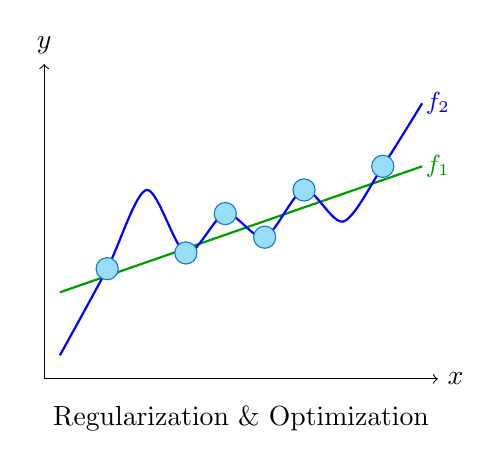
\begin{tikzpicture}[scale=1.0]
    % Axes
    \draw[->] (0,0) -- (5,0) node[right] {$x$};
    \draw[->] (0,0) -- (0,4) node[above] {$y$};

    % f1 (green line) - good linear fit, passes through middle of points
    \draw[thick, green!60!black] (0.2,1.1) -- (4.8,2.7);

    % f2 (blue curve) - passes through all data points
    \draw[thick, blue] plot[smooth, tension=0.5] coordinates {(0.2,0.3) (0.8,1.4) (1.3,2.4) (1.8,1.6) (2.3,2.1) (2.8,1.8) (3.3,2.4) (3.8,2.0) (4.3,2.7) (4.8,3.5)};

    % Data points (smaller light blue circles) - on the curve
    \foreach \x/\y in {0.8/1.4, 1.8/1.6, 2.3/2.1, 2.8/1.8, 3.3/2.4, 4.3/2.7} {
        \fill[cyan!40] (\x,\y) circle (4pt);
        \draw[cyan!60!blue] (\x,\y) circle (4pt);
    }

    % Labels
    \node[green!60!black] at (5.0,2.7) {\small $f_1$};
    \node[blue] at (5.0, 3.5) {\small $f_2$};

    % Title
    \node at (2.5, -0.5) {Regularization \& Optimization};
\end{tikzpicture}
\end{document}
